\subsection{UnSupervised Learning - Finding orientation of xrays}
\label{sec:warmup9}

    This task is an extension of \cref{sec:warmup8}, where we had to find anamolies in xray images. In this task, we have to find orientation of xray images (\cref{sec:warmup3}) using unsupervised learning instead of supervised learning. The same idea will be used to find the orientation as we discussed in \cref{sec:warmup8}, i.e. apply clustering on learned embeddings of xrays.

\subsubsection{Dataset}
  
  For this task, I have merged normal images xrays from \cref{sec:unsupervised-dataset} and xray images from \cref{sec:orienattion-dataset}. The orienation dataset as discussed in \cref{sec:orienattion-dataset} is inversed so that they are constitent with images using which xray reconstruction model was trained in \cref{sec:warmup8}. 

\subsubsection{Result}
 
  The trained xray reconstruction model is used to find embeddings of all the xrays (normal, up, down, right, left). \Cref{fig:unsup-orientation-up,fig:unsup-orienation-right,fig:unsup-orienation-down,fig:unsup-orienation-left} shows the reconstructed xray using original xray. With these images, we can observe that the model is not able to reconstruct xrays if they are not oriented properly, thus their embeddings can be used to cluster the xrays. \Cref{fig:unsup-trained-image} shows reconstructed xray of "normal" image from dataset discussed in \cref{sec:unsupervised-dataset}. The reconstructed image is better than other reconstructed images because the model was trained on this xray.

  The embeddings of all the xrays are used to find $4$ clusters using KMeans clustering algorithm. For testing this learned clusters, I have taken "up" and "normal" xrays as a single class because they are ooriented correctly. The predicted clusters and original clusters are used to calculate rand index which came out to be $0.98$. This rand index means that the embeddings were enough to find cluster the xrays into $4$ clusters. This result can also be visualized using t-SNE in \cref{fig:tSNE}, which shows the perfect $4$ clusters.

  \begin{figure*}[htbp]
    \centering
    \begin{subfigure}{0.49\linewidth}
        \centering
        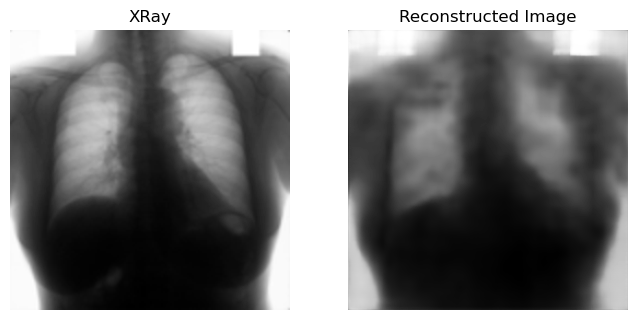
\includegraphics[width=\linewidth]{../plots/unsupervised-orientation/result-up.png}
        \caption{ }
        \label{fig:unsup-orientation-up}
    \end{subfigure}
    \begin{subfigure}{0.49\linewidth}
        \centering
        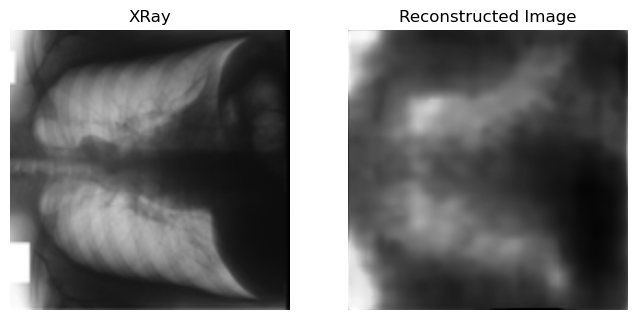
\includegraphics[width=\linewidth]{../plots/unsupervised-orientation/result-right.png}
        \caption{ }
        \label{fig:unsup-orienation-right}
    \end{subfigure}
    \begin{subfigure}{0.49\linewidth}
        \centering
        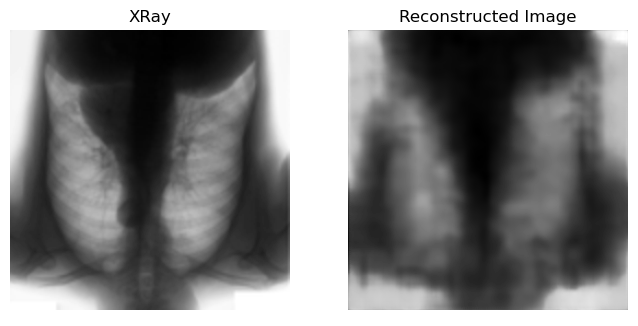
\includegraphics[width=\linewidth]{../plots/unsupervised-orientation/result-down.png}
        \caption{ }
        \label{fig:unsup-orienation-down}
    \end{subfigure}
    \begin{subfigure}{0.49\linewidth}
        \centering
        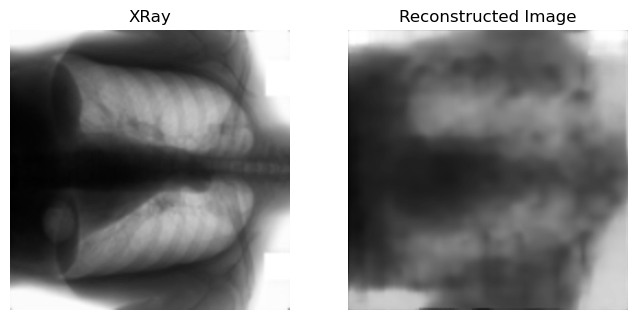
\includegraphics[width=\linewidth]{../plots/unsupervised-orientation/result-left.png}
        \caption{ }
        \label{fig:unsup-orienation-left}
    \end{subfigure}
    \begin{subfigure}{0.49\linewidth}
        \centering
        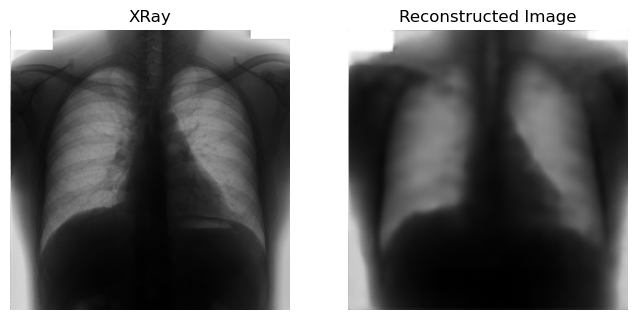
\includegraphics[width=\linewidth]{../plots/unsupervised-orientation/result-trained-xrays.png}
        \caption{ }
        \label{fig:unsup-trained-image}
    \end{subfigure}
  \end{figure*}


\begin{figure}[!htbp]
    \centering
    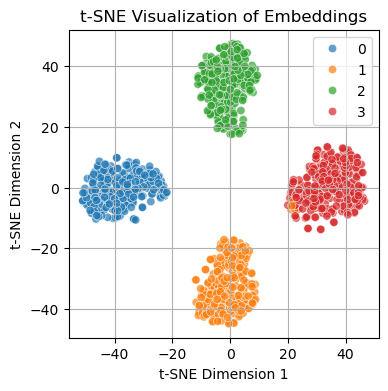
\includegraphics[width=\linewidth]{../plots/unsupervised-orientation/tsne.png}
    \caption{ }
    \label{fig:tSNE}
\end{figure}